%Document-Author: Davide Tommasin
%Document-Date: 2016/05/12
%Document-Description: Manuale Utente del gruppo SWEeneyThreads 

\documentclass[a4paper]{article}
\usepackage[english, italian]{babel}
\usepackage[T1]{fontenc}
\usepackage[utf8]{inputenc}
\usepackage{url}
\usepackage{graphicx}
\usepackage[hidelinks]{hyperref}
\usepackage{booktabs}
\usepackage{eurosym}
\usepackage{tabularx}
\usepackage{pifont}
\usepackage[table]{xcolor}
\usepackage{float}
\usepackage[]{appendix}
\usepackage{ltxtable} 
\usepackage{geometry}
\geometry{margin=1in}
\usepackage{longtable}
\usepackage{multirow}

\graphicspath{{Immagini/}}

\newcolumntype{Y}{>{\centering\arraybackslash}X}
\newcolumntype{s}{>{\hsize=.21\hsize}X}
\newcolumntype{f}{>{\hsize=.37\hsize}X}
\newcolumntype{m}{>{\hsize=.42\hsize}X}
\newcolumntype{t}{>{\hsize=.1\hsize}X}
\newcolumntype{r}{>{\hsize=.3\hsize}X}
\newcolumntype{k}{>{\hsize=.4\hsize}X}

\renewcommand{\abstractname}{Tabella contenuti}

\begin{document}
	
	\begin{titlepage}
		% Defines a new command for the horizontal lines, change thickness here
		\newcommand{\HRule}{\rule{\linewidth}{0.5mm}} 
		\center  
		
		% HEADING SECTION
		\textsc{\LARGE SWEeneyThreads}\\[1.5cm] 
		\textsc{\Large Actorbase}\\[0.5cm] 
		\textsc{\large a NoSQL DB based on the Actor model}\\[0.5cm]
		
		
		% TITLE SECTION
		\HRule \\[0.4cm]
		{ \huge \bfseries User Manual}\\[0.4cm] 
		\HRule \\[1.5cm]
		
		% AUTHOR SECTION
		\begin{minipage}{0.4\textwidth}
			\begin{flushleft} \large
				\emph{Redattori:}\\
				Maino Elia \newline
				Tommasin Davide \\
			\end{flushleft}
		\end{minipage}
		~
		\begin{minipage}{0.4\textwidth}
			\begin{flushright} \large
				\emph{Approvazione:} \\
				\emph{Verifica:} 
			\end{flushright}
		\end{minipage}
		
		%immagine
		\begin{figure}[H]
			\centering
			
\includegraphics[scale=0.8]{sweeney.png}
		\end{figure}
		\begin{center}
			Versione 1.0.2
		\end{center}
		% Date, change the \today to a set date if you want to be precise
		{\large \today}\\[3cm] 
		% Fill the rest of the page with whitespace
		\vfill  
	\end{titlepage}
	
	
	\tableofcontents
	
	\newpage
	\section*{History log}
		\LTXtable{\textwidth}{Tabelle/tabelle_diario_modifiche/tabella_manualeutente_eng.tex}	

	\newpage 
    \section{Introduction}
	\subsection{Document's purpose}
		The present document represents the user manual for the use of \emph{Actorbase}, a No-SQL database. All the user application's features will be described in detail. The manual i dividend into three main sections, related to the main components of the product: Client, Server and Driver.
	\subsection{Product's purpose}
		The project's purpose is the development of a key-value NoSQL Database based on the actor model, with the goal of supply an appropriate technology for the development of modern applications which request very short response time, and which elaborate huges quantities of data. The development will lead to the release of the software under MIT license.
	\subsection{Glossary}
		In order to avoid language ambiguities, and to maximize documents' comprehension, the group wrote \emph{Glossario v2.0.0}. In it will be defined, in a clear and concise way, the terms which could lead to ambiguities or text incomprehensions.
	\subsection{References}
	\subsubsection{Normative}
		\begin{itemize}
			\item \textbf{Norme di progetto:} \emph{Norme di progetto v3.0.0}
			\item \textbf{Capitolato d'appalto Actorbase (C1):} \\ 
			\url{http://www.math.unipd.it/~tullio/IS-1/2015/Progetto/C1p.pdf}
		\end{itemize}
	\newpage

	\section{Actorbase}
	\emph{Actorbase} is a key-value No-SQL database based on the actor model, which guarantees high level of scalability, resilience and performance. It allows to manage easily and flexibly your data, using the mein advantages offered by the actor model, in order to support the development of modern and performing applications.
	\\ \\
	\emph{Actorbase} provides a command line client interface which offers an easy way to handle data as strings, with it it is possible to communicate quickly and intuitively with a server.
	\\ \\
	For more flexible queries it's avaiable the \emph{Scala} driver, integrable with every application.
	\begin{figure}[H]
		\centering
		
\includegraphics[scale=0.4]{actorbaseLogo.png}
		\caption{Actorbase Logo}
	\end{figure}

	\newpage



	\section{System requirements}	
	The correct execution of \emph{Actorbase} is guarantedd on machines that meet the subsequent hardware and software specifications.
	\\ \\
	OS:
	\begin{itemize}
		\item Windows 7 or newer
		\item OS X 10.7 or newer
		\item Ubuntu 14.04 or newer
	\end{itemize}
	Java Virtual Machine (JVM) 8 or newer.
	\\ \\
	RAM:
	\begin{itemize}
		\item Client application: 2GB minimum
		\item Server application: 4GB minimum, 8GB recommended
	\end{itemize}
	There aren't explicit requirements for the processor architecture or speed. Using a very old processor could slow down the system usage.

	\section{Installation}
	\emph{Actorbase} runs on JVM, that's the reason why it doesn't need an installation procedure (just click on the launch icon). 
	\newpage



	\section{Applicativo server}
	L'applicativo server consente di avviare un'istanza \emph{Actorbase} server sulla macchina. Una volta avviato il esso permette ai client di effettuare connessioni alla macchina e di interrogare il database. 
	
	\subsection{Configurazione del server}
	La configurazione della macchina server avviene tramite la modifica del file \texttt{server.conf}. In esso vanno settati indirizzo IP e porta di connessione al server.
	\\
	Nel caso si tentasse di avviare l'applicativo server senza aver definito opportunamente i parametri di configurazione, il server mostrerà un messaggio di errore e non si avvierà.
	
	\subsection{Interfaccia server}
	Una volta modificato il file di configurazione è possibile avviare il server cliccando sull'apposita icona. L'applicativo server fornisce all'utente un'interfaccia da riga di comando che mostra in tempo reale il log delle operazioni effettuate sul server \emph{Actorbase}.  
	\begin{figure}[H]
		\centering
		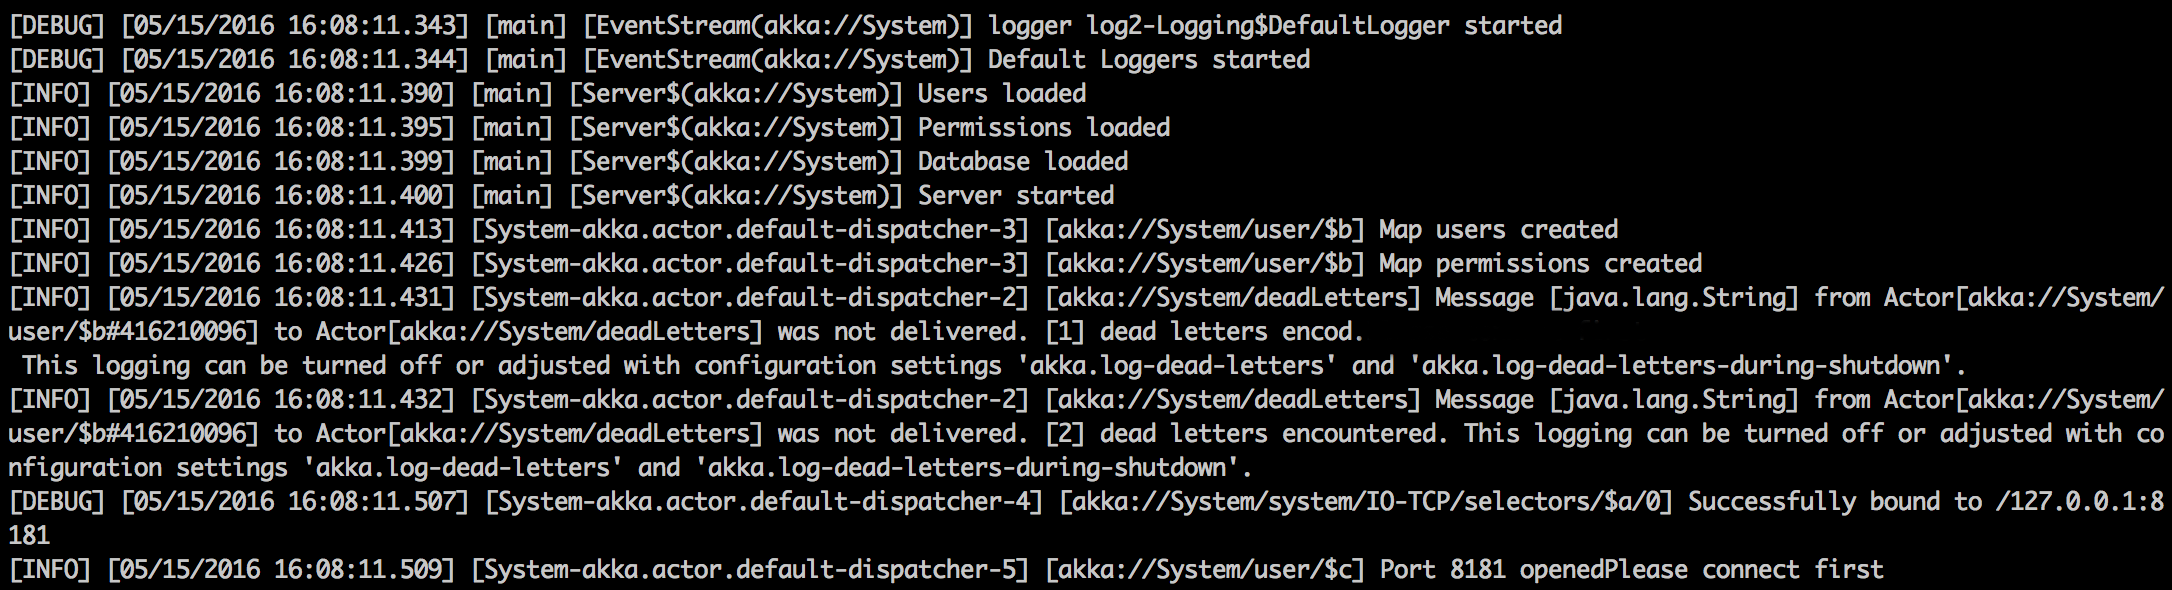
\includegraphics[width=\textwidth]{logServer.png}
		\caption{Interfaccia di log del server}
	\end{figure}
	\newpage
	

	\section{Applicativo client}
	L'applicativo client fornisce all'utente un interfaccia da riga di comando per connettersi ad un server \emph{Actorbase} ed effettuare interrogazioni sul database. Come per il server, l'avvio dell'interfaccia client avviene cliccando sull'apposita icona. Appena avviato il client presenta all'utente un banner di benvenuto seguito da una breve descrizione della configurazione software utilizzata (sistema operativo e JVM).
	\begin{figure}[H]
		\centering
		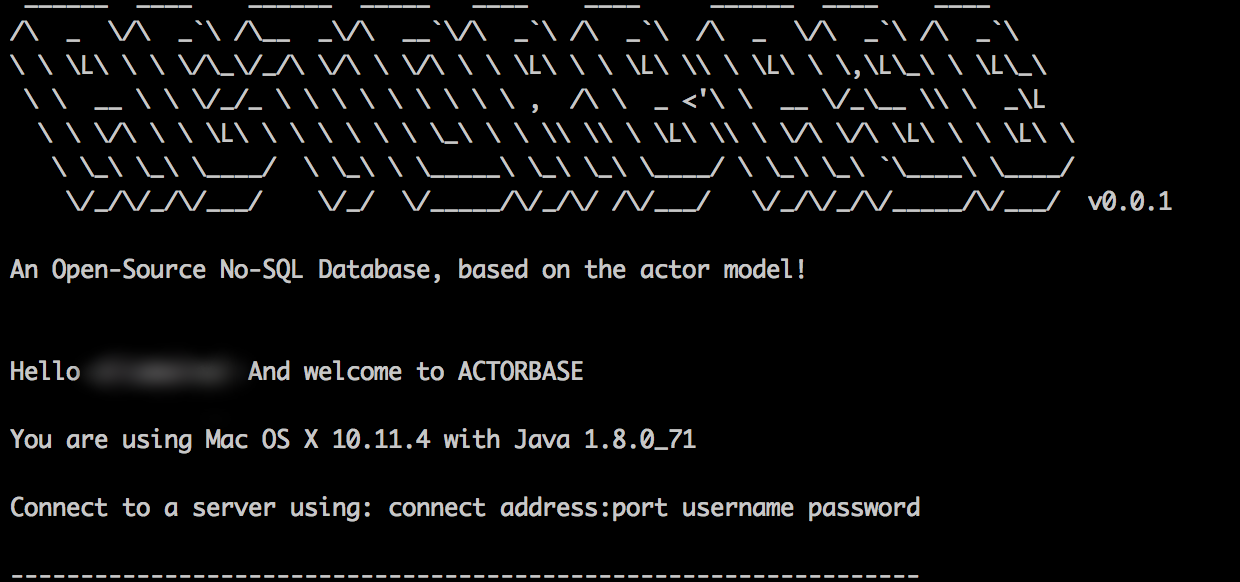
\includegraphics[width=\textwidth]{welcomeClient.png}
		\caption{Informazioni di benvenuto applicativo client}
	\end{figure}
	L'interazione con l'interfaccia avviene tramite l'immissione di comandi testuali, essi possono essere composti da più campi separati da un carattere di spazio.
	
	\subsection{Gestione della connessione}
	Una volta avviato il client per prima cosa è necessario effettuare una connessione ad un server, la gestione della connessione si basa su due comandi: \texttt{connect} e \texttt{disconnect}. L'applicativo client fornito non permette di gestire più connessioni contemporaneamente.
	
	\subsubsection{Comando \texttt{connect}}
	Questo comando permette all'utente di connettersi ad un server, la struttura del comando è la seguente:
	\\ \\
	\texttt{actorbase>	connect indirizzo username password}
	\\ \\
	In particolare l'indirizzo del server deve essere fornito nel formato \texttt{indirizzoServer:porta}. \\ \\
	Nel caso la richiesta di connessione abbia successo l'utente riceve un messaggio di conferma (\texttt{"You are connected!"}), in caso contrario un messaggio di errore (\texttt{"Connection failed!"}).
	
	\subsubsection{Comando \texttt{disconnect}}
	Per effettuare la disconnessione dal server a cui si è connessi è necessario inserire il comando \texttt{disconnect} e premere invio.
	

	\subsection{Aiuto inline}
	\'E possibile ottenere un aiuto per quanto riguarda le operazioni effettuabili, direttamente da riga di comando. Il comando \texttt{help} permette di ottenere sia un aiuto generico che un aiuto specifico.
	
	\subsubsection{Comando \texttt{help} generico}
	Il comando di aiuto generico \texttt{help}, non richiede parametri ulteriori e stampa a video la lista dei comandi di \emph{Actorbase}. Ogni comando è seguito da una breve descrizione che ne illustra il funzionamento.
	
	\subsubsection{Comando \texttt{help} specifico}
	Il comando di aiuto specifico presenta la seguente struttura:
	\\ \\
	\texttt{actorbase>	help nomeComando}
	\\ \\
	Permette di richiedere informazioni per un comando specifico, ottenendone una breve descrizione.
	
	\subsection{Comandi per operazioni a livello server}
	Una volta connesso l'utente si trova a "livello server". A tale livello si possono effettuare operazioni sui database quali:
	\begin{itemize}
		\item Visualizzazione della lista di database
		\item Selezione di un database
		\item Creazione di un database
		\item Rimozione di un database
	\end{itemize}
	
	\subsubsection{Comando \texttt{listdb}}
	Questo comando permette di ottenere, stampata a video, la lista dei database di cui dispone di permessi di accesso (siano essi di visualizzazione o modifica). Tale comando non richiede parametri aggiuntivi.
	\\ \\
	\texttt{actorbase>	listdb}

	\subsubsection{Comando \texttt{selectdb}}
	Questo comando permette di selezionare un database. Una volta selezionato un database l'utente può effettuare operazioni sulle mappe di esso. La struttura del comando di selezione database è la seguente:
	\\ \\
	\texttt{actorbase>	selectdb nomeDatabase}
	\\ \\
	Nel caso l'utente disponga dei permessi necessari alla selezione del database richiesto (\texttt{x}), riceve a video un messaggio di conferma: \texttt{"Database x selected"}. In caso contrario viene riportata un operazione non valida (\texttt{"Invalid operation"}).

	\subsubsection{Comando \texttt{createdb}}
	Questo comando permette di creare un nuovo database col nome specificato, nel caso  un database con tale nome non fosse già presente.
	\\ \\
	\texttt{actorbase>	createdb nomeDatabase}
	\\ \\
	Nel caso esista già un database con il nome inserito la creazione fallisce, l'utente riceve un messaggio di errore: \texttt{"A database with the requested name already exists"}.

	\subsubsection{Comando \texttt{deletedb}}
	Questo comando permette di eliminare un database dal server:
	\\ \\
	\texttt{actorbase>	deletedb nomeDatabase}
	\\ \\
	Nel caso si tenti di rimuovere un database inesistente o di cui non si dispone dei permessi di modifica, l'utente riceve un messaggio di operazione non valida (\texttt{"Invalid operation"}).
	

	\subsection{Comandi per operazioni a livello database}
	Una volta selezionato un database tramite il comando \texttt{selectdb}, l'utente si trova a "livello database". A tale livello si possono effettuare queste operazioni:
	\begin{itemize}
		\item Visualizzazione della lista delle mappe che compongono il database
		\item Selezione di una mappa
		\item Creazione di una mappa
		\item Eliminazione di una mappa
	\end{itemize}

	\subsubsection{Comando \texttt{listmap}}
	Questo comando stampa una lista di tutte le mappe che compongono il database precedentemente selezionato.
	\\ \\
	\texttt{actorbase>	listmap}

	\subsubsection{Comando \texttt{selectmap}}
	Questo comando permette di selezionare una mappa, utilizzando la seguente sintassi:
	\\ \\
	\texttt{actorbase>	selectmap nomeMappa}
	\\ \\
	La selezione viene confermata in caso di successo con il messaggio \texttt{"Map x selected"}, altrimenti si riceve un messaggio di operazione non valida (\texttt{"Invalid operation"}).

	\subsubsection{Comando \texttt{createmap}}
	Questo comando permette di creare una mappa con il nome inserito, all'interno del database selezionato.
	\\ \\
	\texttt{actorbase>	createmap nomeMappa}
	\\ \\
	La creazione viene confermata in caso di successo con il messaggio \texttt{"Map x created"}. Nel caso non si disponga dei permessi di modifica al database, o esista già una mappa con il nome inserito, si riceve un messaggio di operazione non valida (\texttt{"Invalid operation"}).

	\subsubsection{Comando \texttt{deletemap}}
	Questo comando permette di eliminare una mappa dal database selezionato. 
	\\ \\
	\texttt{actorbase>	deletemap nomeMappa}
	\\ \\
	L'eliminazione viene confermata in caso di successo con il messaggio \texttt{"Map x removed"}. Nel caso non si disponga dei permessi di modifica al database, o la mappa richiesta non esista, si riceve un messaggio di operazione non valida (\texttt{"Invalid operation"}).
	

	\subsection{Comandi per operazioni a livello mappa}
	Una volta selezionata una mappa tramite il comando \texttt{selectmap}, l'utente si trova a "livello mappa". A tale livello si possono effettuare queste operazioni:
	\begin{itemize}
		\item Visualizzazione della lista delle chiavi
		\item Ricerca di un item per chiave
		\item Inserimento di un item 
		\item Aggiornamento di un item
		\item Rimozione di un item
	\end{itemize}

	\subsubsection{Comando \texttt{keys}}
	Questo comando permette di visualizzare la lista di tutte le chiavi degli item che compongono la mappa selezionata.
	\\ \\
	\texttt{actorbase>	keys}

	\subsubsection{Comando \texttt{find}}
	Questo comando permette di ottenere il valore di un item della mappa, effettuando la ricerca tramite la sua chiave.
	\\ \\
	\texttt{actorbase>	find key}
	\\ \\
	Nel caso sia presente un item corrispondente alla chiave inserita, si riceve il valore dell'item in formato stringa, stampato a video. Se l'item non viene trovato si riceve un messaggio di errore.
	\subsubsection{Comando \texttt{remove}}
	Questo comando permette di rimuovere un item dalla mappa, ricercandolo tramite la chiave.
	\\ \\
	\texttt{actorbase>	remove key}
	\\ \\
	L'eliminazione viene confermata in caso di successo con il messaggio \texttt{"Item removed"}. Nel caso non si disponga dei permessi di modifica al database, o l'item 
	richiesto non esista, si riceve un messaggio di operazione non valida (\texttt{"Invalid operation"}).

	\subsubsection{Comando \texttt{insert}}
	Questo comando permette di inserire un item (coppia chiave-valore) nella mappa:
	\\ \\
	\texttt{actorbase>	insert key value}
	\\ \\
	L'inserimento viene confermato in caso di successo con il messaggio \texttt{"Item inserted"}. Nel caso non si disponga dei permessi di modifica al database, o sia già presente un item con la chiave inserita, si riceve un messaggio di operazione non valida (\texttt{"Invalid operation"}).
	
	\subsubsection{Comando \texttt{update}}
	Questo comando permette di aggiornare un item dalla mappa, ricercandolo tramite la chiave e inserendo il valore aggiornato.
	\\ \\
	\texttt{actorbase>	update key value}
	\\ \\
	L'aggiornamento viene confermato in caso di successo con il messaggio \texttt{"Item updated"}. Nel caso non si disponga dei permessi di modifica al database, o l'item 
	richiesto non esista, si riceve un messaggio di operazione non valida (\texttt{"Invalid operation"}).
			
	\cleardoublepage
	\addcontentsline{toc}{section}{\listfigurename}
	\listoffigures
	
	\cleardoublepage
	\addcontentsline{toc}{section}{\listtablename}
	\listoftables
		
\end{document}